\ohead{5. Mai 2011}
\section{Beispiele (\glqq zum Warmwerden\grqq)}
\subsection{Randomized Quicksort}
\begin{algorithm}
	\caption{Algorithmus randQS ($S$: Array aus $n$ verschiedenen Zahlen)}
	\vspace{0.4cm}
	\begin{enumerate}
		\setlength{\itemsep}{2pt}
		\setlength{\parskip}{2pt}
		\setlength{\parsep}{2pt}
		\item Wähle ein $y$ aus $S$ ($y$ heißt Pivotelement) u.a.r.\ (\textit{uniformly at random})
		\item $S_1 := \{ x \in S\ |\ x < y \} \quad S_2 := \{ x \in S\ |\ x > y \}$
		\item \textbf{if} $S_1 \not= \emptyset$ \textbf{then} randQS($S_1$)
		\item print $y$
		\item \textbf{if} $S_2 \not= \emptyset$ \textbf{then} randQS($S_2$)
	\end{enumerate}
\end{algorithm}
Wir messen die Laufzeit in der Anzahl der Vergleiche auf Schlüsseln.
\subsubsection{\textit{worst-case}-Szenario}
\begin{center}
\renewcommand\arraystretch{1.3}
\begin{tabular}{ccccccc|c|c}
	&&&&&&& \# Vergleiche & Wahrscheinlichkeit \\
	$1$&$2$&$3$&$4$&$5$&$6$&$7$&$6$&$\frac{1}{7}$\\
	&$2$&$3$&$4$&$5$&$6$&$7$&$5$&$\frac{1}{6}$\\
	&&&$\ddots$&&&&&\\
	&&&&&$6$&$7$&$1$&$\frac{1}{2}$\\
	&&&&&&$7$&$0$&$1$
\end{tabular}
\renewcommand\arraystretch{2.5}
\begin{tabular}{rl}
	Gesamtzahl der Vergleiche: & $\displaystyle \sum_{i=1}^{n-1} i = \frac{n(n-1)}{2} \in \Theta(n^2)$ \\
	Gesamtwahrscheinlichkeit: & $\displaystyle \prod_{i=1}^{n} \frac{1}{i} = \frac{1}{n!}$
\end{tabular}
\end{center}
\subsubsection{Probabilistische Laufzeitanalyse}
Wir bestimmen die erwartete Laufzeit: Sei $s_i$ der Schlüssel mit Rang $i$
($i$-t-kleinster Schlüssel). Wir definieren für $1 \leq i < j \leq n$ folgende
Zufallsvariable:
\[
  X_{ij} = \begin{cases} 1 & \text{falls der Algor. $s_i$ und $s_j$ vergleicht} \\
	  0 & \text{sonst} \end{cases}
\]
Die Gesamtzahl der Vergleiche ist $\sum_{i=1}^n \sum_{j=i+1}^n X_{ij}$.
Definiere $p_{ij} = P\left[X_{ij} = 1\right]$. Der Erwartungswert ist damit
wegen $E\left[X_{ij}\right] = 0 \cdot P\left[X_{ij} = 0\right] + 1 \cdot
P\left[X_{ij} = 1\right]$ gleich
\[
  E\left[\sum_{i=1}^n \sum_{j=i+1}^n X_{ij}\right] = \sum_{i=1}^n
  \sum_{j=i+1}^n E\left[X_{ij}\right] = \sum_{i<j} p_{ij}.
\]

Anhand folgenden Beispiels soll eine äquivalente Formulierung für $X_{ij}$
gezeigt werden (fettgedruckte Zahlen sind die in diesem Schritt neu gewählten
Pivotelemente, unterstrichene Zahlen entsprechen den Pivotelementen der
vorhergehenden Schritte):

\vspace{0.5cm}
\begin{minipage}{0.6\linewidth}
\renewcommand\arraystretch{1.3}
\centering
\begin{tabular}{ccccccc}
	$\mathbf{3}$ & $5$ & $2$ & $1$ & $5$ & $7$ & $6$ \\
	$2$ & $\mathbf{1}$ & $\underline{3}$ & $4$ & $\mathbf{5}$ & $7$ & $6$ \\
	$\underline{1}$ & $\mathbf{2}$ & $\underline{3}$ & $\mathbf{4}$ & $\underline{5}$ & $7$ & $\mathbf{6}$ \\
	$\underline{1}$ & $\underline{2}$ & $\underline{3}$ & $\underline{4}$ & $\underline{5}$ & $\underline{6}$ & $\mathbf{7}$
\end{tabular}
\end{minipage}\hfill\begin{minipage}{0.3\linewidth}
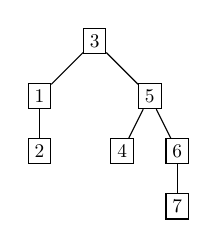
\begin{tikzpicture}[scale=0.7,level distance=10mm,level/.style={sibling distance=20mm/#1}]
	\tikzstyle{every node}=[draw,scale=0.7]
	\node (a){$3$}
	child {node (b) {$1$} child { node (c) {$2$} }}
	child {node (d) {$5$} child { node (e) {$4$} } child { node (f) {$6$} child { node (g) {$7$} } } };
\end{tikzpicture}
\end{minipage}
\vspace{0.5cm}

Die Schlüssel $s_i$ und $s_j$ werden also genau dann miteinander verglichen,
wenn nur $s_i$ oder $s_j$ als erstes aus $S_{ij} = \{ s_i, \dots, s_j \}$ als
Pivotelement gewählt werden:
\[
  X_{ij} = \begin{cases} 1 & \text{falls $s_j$-Knoten Nachfolger des
  $s_i$-Knoten oder umgekehrt} \\ 0 & \text{sonst} \end{cases}
\]
\begin{align*}
  \Rightarrow p_{ij} &= P\left[s_i \text{ wird als erstes Pivotelement aus $S_{ij}$ gewählt}\right] \\
  &+ P\left[s_j \text{ wird als erstes Pivotelement aus $S_{ij}$ gewählt}\right] = \frac{2}{j-i+1}
\end{align*}
Unter Verwendung der Eigenschaft der harmonischen Reihe $\ln(i+1) \leq H_i =
\sum_{k=1}^i \frac{1}{k} \leq 1 + \ln i$ ergibt sich für den Erwartungswert
\begin{align*}
	\sum_{i<j} p_{ij} &= \sum_{i=1}^n \sum_{j=1}^n \frac{2}{j-i+1} = 2 \cdot \sum_{i=2}^n \sum_{j=2}^i \frac{1}{j} \\
			  &\leq 2 \cdot \sum_{i=1}^n \left(H_i - 1\right) \leq 2 n \ln n = (2 \ln 2) n \log_2 n \approx 1.386\dots n \log_2 n
\end{align*}
\renewcommand\arraystretch{1.5}
\begin{tabular}{r|ccccccc}
	& & $j = 2$ & 3 & 4 & $\cdots$ & $n-1$ & $n$ \\
	\hline
	$i = 1$ & $0$ & $\frac{2}{2}$ & $\frac{2}{3}$ & $\frac{2}{4}$ & $\cdots$ & $\frac{2}{n-1}$ & $\frac{2}{n}$ \\
	$2$ && $0$ & $\frac{2}{2}$ & $\frac{2}{3}$ & $\cdots$ & $\cdots$ & $\frac{2}{n-1}$ \\
	$3$ &&& $0$ & $\frac{2}{2}$ & $\cdots$ & $\cdots$ & $\frac{2}{n-2}$
\end{tabular}
